\section{Dirichlet分布}
\label{sec:mvd-dirichlet}

甜品店的三种口味，选择概率$(0.5,0.3,0.2)$并不是一成不变的：天气、节日、新品都会让这天的偏好与那天不同。若把每天的偏好本身看成随机的，就得到一个随机的比例向量$\bm{P}=(P_1,P_2,P_3)^{\top}$，分量非负、和为$1$。一份混合物中各成分所占的比例，也是这样的对象。

这类对象与计数不同。多项分布中$\bm{p}$是给定的参数，随机的是计数；这里随机的是比例本身。两层可以叠加：先随机产生当天的偏好$\bm{P}$，再在给定$\bm{P}$时产生多项计数。本节只讨论比例的分布本身。由观测到的计数反过来更新对比例的认识，属于统计推断，归卷八。

一元时，第~\ref{chap:common-distributions}章的Beta分布描述$(0,1)$中的一个随机比例，另一类的比例就是它的补数。Dirichlet分布把它推广到$d$个类别。我们先说明它住在什么地方、密度相对于什么坐标，再用独立Gamma变量构造它，最后计算均值与协方差。

\subsection{单纯形上的密度}
\label{sec:mvd-dirichlet-density}

\paragraph{取值范围}
$d$个类别的比例向量取值于\term{标准单纯形}（standard simplex）
\[
 \Delta_{d-1}=\Bigl\{\bm{p}\in\mathbb{R}^{d}:\ p_i\geq0,\ \sum_{i=1}^{d}p_i=1\Bigr\} .
\]
$d=3$时它是$\mathbb{R}^{3}$中以三个坐标向量为顶点的三角形，图~\ref{fig:mvd-simplex}左侧；下标$d-1$是它的维数。

$\Delta_{d-1}$落在超平面$\sum_ip_i=1$里，$d$维体积为$0$，所以$\bm{P}$不可能有普通的$d$维密度，理由与退化高斯相同。办法是只用前$d-1$个分量作坐标，最后一个由$p_d=1-p_1-\cdots-p_{d-1}$确定。这些自由坐标取值于
\[
 T_{d-1}=\Bigl\{(p_1,\ldots,p_{d-1}):\ p_i>0,\ \sum_{i=1}^{d-1}p_i<1\Bigr\} ,
\]
$d=3$时是平面上的直角三角形，图~\ref{fig:mvd-simplex}右侧。密度就是$(P_1,\ldots,P_{d-1})$在$T_{d-1}$上的普通密度。

\begin{BookInlineFigure}
  \centering
  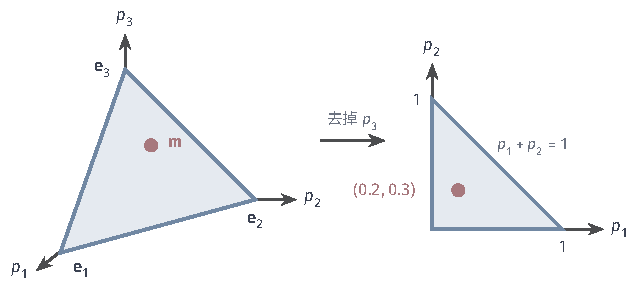
\includegraphics[width=109mm]{figures/07-probability/01-elementary-probability/tikz/mvd-simplex/figure.pdf}
  \caption{三个类别的比例。左：$\mathbb{R}^{3}$中的标准单纯形$\Delta_2$（浅蓝三角形），顶点为$\bm{e}_1,\bm{e}_2,\bm{e}_3$，红点$\bm{m}=(0.2,0.3,0.5)$。右：去掉$p_3$后的自由坐标区域$T_2$，红点是$\bm{m}$的像$(0.2,0.3)$。}
  \label{fig:mvd-simplex}
\end{BookInlineFigure}

\paragraph{密度与归一化}
Beta密度$t^{\alpha_1-1}(1-t)^{\alpha_2-1}$在$t$接近$0$时由$\alpha_1$控制，接近$1$时由$\alpha_2$控制。多个类别时，对每个比例都放一个这样的幂因子。

\begin{definition}[Dirichlet分布]
\label{def:mvd-dirichlet}
设$d\geq2$，$\bm{\alpha}=(\alpha_1,\ldots,\alpha_d)^{\top}$的各分量$\alpha_i>0$，记$\alpha_0=\alpha_1+\cdots+\alpha_d$。若随机向量$\bm{P}$取值于$\Delta_{d-1}$，且$(P_1,\ldots,P_{d-1})$在$T_{d-1}$上有密度
\begin{equation}
 f(p_1,\ldots,p_{d-1})=\frac{\Gamma(\alpha_0)}{\Gamma(\alpha_1)\cdots\Gamma(\alpha_d)}\prod_{i=1}^{d}p_i^{\alpha_i-1},\qquad p_d=1-\sum_{i=1}^{d-1}p_i ,
 \label{eq:mvd-dirichlet-density}
\end{equation}
则称$\bm{P}$服从参数为$\bm{\alpha}$的\term{Dirichlet分布}（Dirichlet distribution），记为$\bm{P}\sim\operatorname{Dir}(\bm{\alpha})$。
\end{definition}

$d=2$时，$P_1$在$(0,1)$上的密度是$\Gamma(\alpha_1+\alpha_2)/(\Gamma(\alpha_1)\Gamma(\alpha_2))\cdot p_1^{\alpha_1-1}(1-p_1)^{\alpha_2-1}$，就是$\operatorname{Beta}(\alpha_1,\alpha_2)$。第~\ref{chap:common-distributions}章的归一化等价于Beta积分
\[
 \int_0^{1}t^{a-1}(1-t)^{b-1}\,\mathrm{d}t=\frac{\Gamma(a)\Gamma(b)}{\Gamma(a+b)},\qquad a,b>0 .
\]
一般的$d$需要验证式~\eqref{eq:mvd-dirichlet-density}的积分为$1$，下面用归纳法从Beta积分推出。

\begin{lemma}[Dirichlet积分]
\label{lem:mvd-dirichlet-integral}
对$d\geq2$及正数$\alpha_1,\ldots,\alpha_d$，
\begin{equation}
 \int_{T_{d-1}}\prod_{i=1}^{d}p_i^{\alpha_i-1}\,\mathrm{d}p_1\cdots\mathrm{d}p_{d-1}=\frac{\Gamma(\alpha_1)\cdots\Gamma(\alpha_d)}{\Gamma(\alpha_0)} ,
 \label{eq:mvd-dirichlet-integral}
\end{equation}
其中$p_d=1-\sum_{i<d}p_i$。
\end{lemma}

\begin{proof}
$d=2$就是Beta积分。设结论对$d-1$成立，$d\geq3$。被积函数非负，可以先对$p_{d-1}$积分。固定$p_1,\ldots,p_{d-2}$，记$s=p_1+\cdots+p_{d-2}<1$，则$p_{d-1}$的范围是$(0,1-s)$，$p_d=1-s-p_{d-1}$。

令$p_{d-1}=(1-s)t$，$t\in(0,1)$，则$p_d=(1-s)(1-t)$，$\mathrm{d}p_{d-1}=(1-s)\,\mathrm{d}t$，于是
\[
 \int_0^{1-s}p_{d-1}^{\alpha_{d-1}-1}p_d^{\alpha_d-1}\,\mathrm{d}p_{d-1}=(1-s)^{\alpha_{d-1}+\alpha_d-1}\,\frac{\Gamma(\alpha_{d-1})\Gamma(\alpha_d)}{\Gamma(\alpha_{d-1}+\alpha_d)} .
\]

剩下对$(p_1,\ldots,p_{d-2})\in T_{d-2}$的积分，被积函数是$\prod_{i\leq d-2}p_i^{\alpha_i-1}$乘以$(1-s)^{(\alpha_{d-1}+\alpha_d)-1}$。这正是$d-1$个类别、参数为$(\alpha_1,\ldots,\alpha_{d-2},\alpha_{d-1}+\alpha_d)$时的同类积分，参数之和仍为$\alpha_0$。由归纳假设，它等于
\[
 \frac{\Gamma(\alpha_1)\cdots\Gamma(\alpha_{d-2})\,\Gamma(\alpha_{d-1}+\alpha_d)}{\Gamma(\alpha_0)} .
\]
与前一个因子相乘，$\Gamma(\alpha_{d-1}+\alpha_d)$消去，得到式~\eqref{eq:mvd-dirichlet-integral}。
\end{proof}

证明顺带说明了一件事：把最后两类合并，$(P_1,\ldots,P_{d-2},P_{d-1}+P_d)$服从$\operatorname{Dir}(\alpha_1,\ldots,\alpha_{d-2},\alpha_{d-1}+\alpha_d)$，因为对$p_{d-1}$积分后剩下的正是这个分布的密度。式~\eqref{eq:mvd-dirichlet-density}在$d$个分量间是对称的（换用另一组$d-1$个自由坐标是行列式为$\pm1$的线性换元），所以任意几类都可以合并，参数相加。反复合并，只留下第$i$类与“其余各类”，就得到边缘分布
\begin{equation}
 P_i\sim\operatorname{Beta}(\alpha_i,\ \alpha_0-\alpha_i) .
 \label{eq:mvd-dirichlet-marginal}
\end{equation}
这与多项计数合并类别后仍为多项分布是同一种结构。

\paragraph{一个例子}
取$\bm{\alpha}=(2,3,5)^{\top}$，$\alpha_0=10$。归一化常数是
\[
 \frac{\Gamma(10)}{\Gamma(2)\Gamma(3)\Gamma(5)}=\frac{9!}{1!\cdot2!\cdot4!}=\frac{362880}{48}=7560 .
\]
在$\bm{p}=(0.2,0.3,0.5)$处，密度为
\[
 7560\times0.2\times0.3^{2}\times0.5^{4}=7560\times0.001125\approx8.51 .
\]
各$\alpha_i>1$时，在约束$\sum_ip_i=1$下最大化$\ln f=\text{常数}+\sum_i(\alpha_i-1)\ln p_i$，Lagrange条件要求$(\alpha_i-1)/p_i$对各$i$相同，所以密度的最高点在$p_i=(\alpha_i-1)/(\alpha_0-d)$。这里是$(1,2,4)/7\approx(0.14,0.29,0.57)$，与均值$(0.2,0.3,0.5)$不同。

\paragraph{参数小于一的边界}
$\alpha_i<1$时因子$p_i^{\alpha_i-1}$在$p_i\to0$时趋于无穷，密度在面$p_i=0$附近无界。图~\ref{fig:mvd-dirichlet-density}(c)取$\bm{\alpha}=(0.5,0.5,0.5)^{\top}$，颜色向三条边加深。这不意味着边界上有正概率：密度只描述单位面积上的概率，无界的密度仍可以积分为有限值。

用边缘分布可以算得很具体。$\bm{\alpha}=(0.5,0.5,0.5)^{\top}$时，由式~\eqref{eq:mvd-dirichlet-marginal}，$P_1\sim\operatorname{Beta}(1/2,1)$，密度为$\tfrac12t^{-1/2}$，于是
\[
 \mathbb{P}(P_1\leq\varepsilon)=\int_0^{\varepsilon}\tfrac12t^{-1/2}\,\mathrm{d}t=\sqrt\varepsilon .
\]
$\varepsilon=0.01$时这个概率是$0.1$，比均匀分布下大得多，说明比例确实偏爱靠近边界；但它随$\varepsilon\to0$趋于$0$，所以$\mathbb{P}(P_1=0)=0$，边界上没有点质量。一般地，$\mathbb{P}(P_i\leq\varepsilon)$与$\varepsilon^{\alpha_i}$同阶。

\begin{BookInlineFigure}
  \centering
  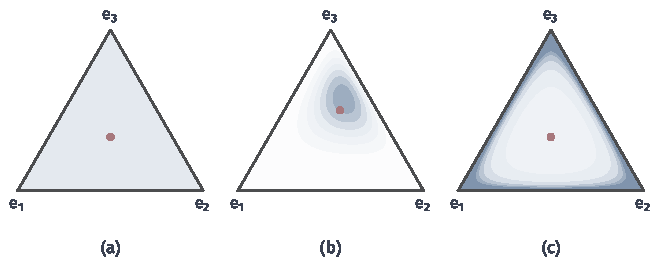
\includegraphics[width=112mm]{figures/07-probability/01-elementary-probability/matplotlib/mvd-dirichlet-density/figure.pdf}
  \caption{Dirichlet密度画在等边三角形上，顶点$\bm{e}_i$对应$p_i=1$；颜色由白到蓝表示密度由小到大，各图色阶分别设定。(a)$\bm{\alpha}=(1,1,1)$，密度恒为$2$。(b)$\bm{\alpha}=(2,3,5)$。(c)$\bm{\alpha}=(0.5,0.5,0.5)$，密度向三条边增大（颜色在$3$处截断）。红点是均值$\bm{\alpha}/\alpha_0$。}
  \label{fig:mvd-dirichlet-density}
\end{BookInlineFigure}

$\bm{\alpha}=(1,1,1)^{\top}$时密度恒为$\Gamma(3)=2$，是$T_2$上的均匀分布：三角形$T_2$的面积是$1/2$。$\alpha_i$都大于$1$时，密度在内部有唯一的峰，在边界上趋于$0$，图~\ref{fig:mvd-dirichlet-density}(b)。

\subsection{Gamma归一化}
\label{sec:mvd-gamma-normalization}

比例最自然的来源是“各部分的量除以总量”。设三种成分的量相互独立，各自是正的随机变量，把它们除以总量，就得到一个随机比例。量取Gamma分布时，比例恰好是Dirichlet分布。

\begin{theorem}[Gamma归一化]
\label{thm:mvd-gamma-normalization}
设随机变量$G_i\sim\operatorname{Gamma}(\alpha_i,\beta)$，$i=1,\ldots,d$，相互独立，速率$\beta>0$相同。令$T=G_1+\cdots+G_d$，则
\begin{equation}
 \bm{P}=\Bigl(\frac{G_1}{T},\ldots,\frac{G_d}{T}\Bigr)^{\top}\sim\operatorname{Dir}(\bm{\alpha}) ,
 \label{eq:mvd-gamma-normalization}
\end{equation}
并且$T\sim\operatorname{Gamma}(\alpha_0,\beta)$，$T$与$\bm{P}$相互独立。
\end{theorem}

证明要求出$(T,P_1,\ldots,P_{d-1})$的联合密度，这是一个$d$维到$d$维的可逆换元，在第~\ref{chap:random-variable-transformations}章用总量与比例的变换完成。这里先核对定理中各项的含义。

\paragraph{取值范围与参数}
每个$G_i$以概率$1$为正，所以$T>0$，各$P_i\in(0,1)$，且$P_1+\cdots+P_d=1$：$\bm{P}$确实落在单纯形内部。第$i$类的形状参数$\alpha_i$原样成为Dirichlet参数的第$i$个分量。形状参数越大，$G_i$越倾向于取大值，第$i$类在总量中占的比例也越大，这与下面算出的均值$\alpha_i/\alpha_0$一致。

\paragraph{共同速率被消去}
速率只是一个共同的单位。若$G\sim\operatorname{Gamma}(\alpha,\beta)$，对$x>0$代换$h=\beta g$，
\[
 \mathbb{P}(\beta G\leq x)=\int_0^{x/\beta}\frac{\beta^{\alpha}g^{\alpha-1}\mathrm{e}^{-\beta g}}{\Gamma(\alpha)}\,\mathrm{d}g=\int_0^{x}\frac{h^{\alpha-1}\mathrm{e}^{-h}}{\Gamma(\alpha)}\,\mathrm{d}h ,
\]
所以$\beta G\sim\operatorname{Gamma}(\alpha,1)$。于是可以写$G_i=H_i/\beta$，$H_i\sim\operatorname{Gamma}(\alpha_i,1)$相互独立，而
\[
 \frac{G_i}{T}=\frac{H_i/\beta}{\sum_jH_j/\beta}=\frac{H_i}{\sum_jH_j} .
\]
比例与$\beta$无关。共同速率只改变各部分的单位，不改变各部分之间的相对大小。

如果各$G_i$的速率不同，速率就不能约去，比例一般不是Dirichlet分布。图~\ref{fig:mvd-gamma-normalization}以$\bm{g}=(1.2,0.6,2.2)$为例：总量为$4$，比例为$(0.3,0.15,0.55)$；所有量同时加倍（相当于速率减半）后总量为$8$，比例不变。

\begin{BookInlineFigure}
  \centering
  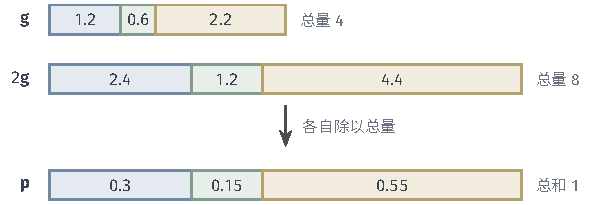
\includegraphics[width=97mm]{figures/07-probability/01-elementary-probability/tikz/mvd-gamma-normalization/figure.pdf}
  \caption{Gamma归一化的一个取值。三种成分的量$\bm{g}=(1.2,0.6,2.2)$（第一行），全部加倍得$2\bm{g}$（第二行）；除以各自的总量$4$与$8$后得到同一个比例向量$\bm{p}=(0.3,0.15,0.55)$（第三行）。}
  \label{fig:mvd-gamma-normalization}
\end{BookInlineFigure}

\paragraph{比例之间为什么相关}
$G_1,\ldots,G_d$相互独立，比例却通过共同的分母联系在一起：某一类的量偏大，总量随之变大，其他各类的比例就被压低。这与多项计数的负相关来源相似，都是“总和固定”在起作用。

定理~\ref{thm:mvd-gamma-normalization}还给出了生成Dirichlet样本的方法：独立地生成$d$个Gamma变量，第$i$个的形状参数为$\alpha_i$、速率为$1$，再各自除以它们的和。下一小节图中的模拟样本就是这样得到的，更多的生成方法在第~\ref{chap:sample-generation}章讨论。

\subsection{均值与协方差}
\label{sec:mvd-dirichlet-moments}

Dirichlet积分把矩的计算变成参数的移位：乘以$p_i$，只是把$\alpha_i$加$1$。对非负整数$r_1,\ldots,r_d$，记$r=\sum_ir_i$，由式~\eqref{eq:mvd-dirichlet-integral}，
\begin{equation}
 \mathbb{E}\Bigl[\prod_{i=1}^{d}P_i^{r_i}\Bigr]=\frac{\Gamma(\alpha_0)}{\Gamma(\alpha_0+r)}\prod_{i=1}^{d}\frac{\Gamma(\alpha_i+r_i)}{\Gamma(\alpha_i)} .
 \label{eq:mvd-dirichlet-moments}
\end{equation}
这里的乘积包括$P_d$，因为$p_d$在被积函数中本来就以幂的形式出现。

\begin{theorem}[Dirichlet的均值与协方差]
\label{thm:mvd-dirichlet-cov}
设$\bm{P}\sim\operatorname{Dir}(\bm{\alpha})$，记$m_i=\alpha_i/\alpha_0$，$\bm{m}=(m_1,\ldots,m_d)^{\top}$。则$\mathbb{E}[\bm{P}]=\bm{m}$，并且
\begin{equation}
 \operatorname{Cov}(\bm{P})=\frac{1}{\alpha_0+1}\bigl(\operatorname{diag}(\bm{m})-\bm{m}\bm{m}^{\top}\bigr) ,
 \label{eq:mvd-dirichlet-cov}
\end{equation}
即$\operatorname{Var}(P_i)=m_i(1-m_i)/(\alpha_0+1)$，$i\neq j$时$\operatorname{Cov}(P_i,P_j)=-m_im_j/(\alpha_0+1)$。
\end{theorem}

\begin{proof}
在式~\eqref{eq:mvd-dirichlet-moments}中用$\Gamma(x+1)=x\Gamma(x)$。只取$r_i=1$，得$\mathbb{E}[P_i]=\alpha_i/\alpha_0$。取$r_i=2$或$r_i=r_j=1$（$i\neq j$），得
\[
 \mathbb{E}[P_i^{2}]=\frac{\alpha_i(\alpha_i+1)}{\alpha_0(\alpha_0+1)},\qquad \mathbb{E}[P_iP_j]=\frac{\alpha_i\alpha_j}{\alpha_0(\alpha_0+1)} .
\]

方差为
\[
 \begin{aligned}
  \operatorname{Var}(P_i)&=\frac{\alpha_i(\alpha_i+1)}{\alpha_0(\alpha_0+1)}-\frac{\alpha_i^{2}}{\alpha_0^{2}}
  =\frac{\alpha_i\bigl[(\alpha_i+1)\alpha_0-\alpha_i(\alpha_0+1)\bigr]}{\alpha_0^{2}(\alpha_0+1)}\\
  &=\frac{\alpha_i(\alpha_0-\alpha_i)}{\alpha_0^{2}(\alpha_0+1)} ,
 \end{aligned}
\]
即$m_i(1-m_i)/(\alpha_0+1)$。协方差为
\[
 \operatorname{Cov}(P_i,P_j)=\frac{\alpha_i\alpha_j}{\alpha_0(\alpha_0+1)}-\frac{\alpha_i\alpha_j}{\alpha_0^{2}}=-\frac{\alpha_i\alpha_j}{\alpha_0^{2}(\alpha_0+1)} .
\]
\end{proof}

用边缘分布核对一下。由式~\eqref{eq:mvd-dirichlet-marginal}，$P_i\sim\operatorname{Beta}(\alpha_i,\alpha_0-\alpha_i)$；按第~\ref{chap:common-distributions}章的Beta公式，均值是$\alpha_i/\alpha_0$，方差是
\[
 \frac{\alpha_i(\alpha_0-\alpha_i)}{\alpha_0^{2}(\alpha_0+1)} ,
\]
与定理一致。也可以用定理~\ref{thm:mvd-gamma-normalization}核对均值：$G_i=TP_i$，而$T$与$\bm{P}$独立，所以
\[
 \frac{\alpha_i}{\beta}=\mathbb{E}[G_i]=\mathbb{E}[T]\,\mathbb{E}[P_i]=\frac{\alpha_0}{\beta}\,\mathbb{E}[P_i] ,
\]
即$\mathbb{E}[P_i]=\alpha_i/\alpha_0$。

取$\bm{\alpha}=(2,3,5)^{\top}$，$\bm{m}=(0.2,0.3,0.5)^{\top}$，$\alpha_0+1=11$。代入式~\eqref{eq:mvd-dirichlet-cov}，
\[
 \operatorname{Cov}(\bm{P})=\frac{1}{11}\begin{bmatrix}0.16&-0.06&-0.10\\-0.06&0.21&-0.15\\-0.10&-0.15&0.25\end{bmatrix}\approx\begin{bmatrix}0.0145&-0.0055&-0.0091\\-0.0055&0.0191&-0.0136\\-0.0091&-0.0136&0.0227\end{bmatrix} .
\]
三个比例两两负相关，每行之和为$0$。

\paragraph{总和约束与奇异协方差}
行和为$0$的原因与多项分布相同：$\operatorname{diag}(\bm{m})-\bm{m}\bm{m}^{\top}$乘以$\bm{1}$得$\bm{m}-\bm{m}=\bm{0}$，对应$\operatorname{Var}(P_1+\cdots+P_d)=0$。各$m_i>0$，所以与多项分布一样，这个矩阵的秩是$d-1$，与单纯形的维数一致。所有比例两两负相关：一个比例变大，其余比例的总和必须变小。

\paragraph{集中程度}
式~\eqref{eq:mvd-dirichlet-cov}把参数分成两部分：方向$\bm{m}=\bm{\alpha}/\alpha_0$决定均值，总和$\alpha_0$决定比例围绕均值的集中程度，协方差与$\alpha_0+1$成反比。$\alpha_0$因此称为\term{集中参数}（concentration parameter）。

固定$\bm{m}=(0.2,0.3,0.5)^{\top}$，让$\alpha_0$取$1,10,100$，$\operatorname{Var}(P_1)=0.16/(\alpha_0+1)$分别是$0.08$、$0.0145$、$0.0016$。图~\ref{fig:mvd-dirichlet-concentration}画出对应的样本。$\alpha_0=1$时各$\alpha_i<1$，样本挤到边和顶点附近，即某一两类占了绝大部分；$\alpha_0=100$时样本紧紧围着$\bm{m}$。

\begin{BookInlineFigure}
  \centering
  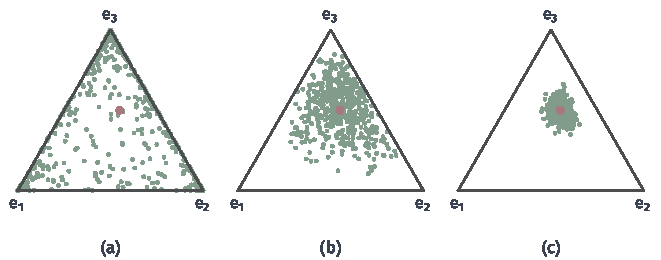
\includegraphics[width=112mm]{figures/07-probability/01-elementary-probability/matplotlib/mvd-dirichlet-concentration/figure.pdf}
  \caption{均值固定为$\bm{m}=(0.2,0.3,0.5)$（红点）、集中参数不同的Dirichlet样本，各$500$个，用Gamma归一化生成。(a)$\alpha_0=1$，种子$51$；(b)$\alpha_0=10$，种子$52$；(c)$\alpha_0=100$，种子$53$。三组样本中$P_1$的样本方差分别约为$0.089$、$0.014$、$0.0016$。}
  \label{fig:mvd-dirichlet-concentration}
\end{BookInlineFigure}
